%\pagecolor{gray} 
\graphicspath{ {../choicungbi/gapvacathinh/} }
\begingroup
\AddToShipoutPicture*{\put(80,540){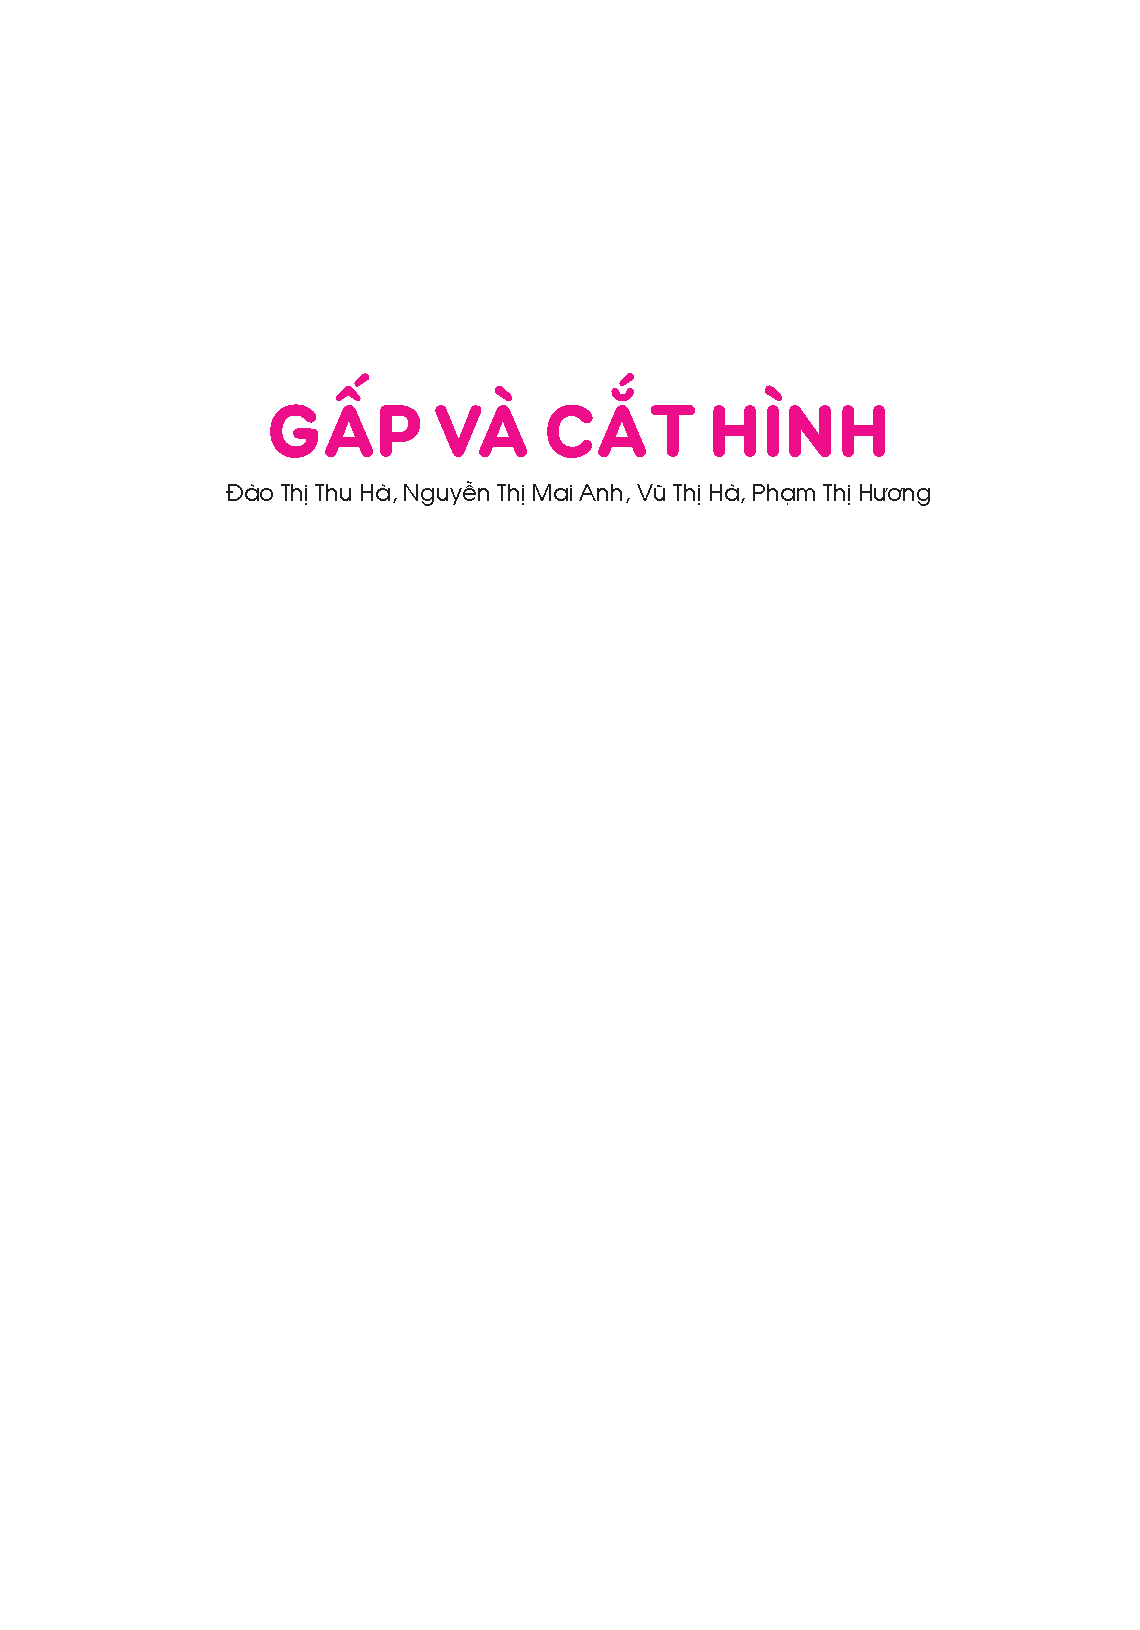
\includegraphics[scale=0.5]{../gapvacathinh/toancuabi}}} % %Image background
\centering
\endgroup
	
\vspace*{1pt}
	
Từ khi còn học mầm non, Bi  đã được làm quen với việc dùng kéo để cắt giấy, tạo ra nhiều hình khác nhau. Từ ngày biết về tính đối xứng, Bi đã áp dụng nó vào trò chơi cắt hình.
Nhiều hình tưởng phức tạp, nhưng mình sẽ cắt được nhanh hơn, nếu quan sát kỹ.
\vskip 0.1cm
Nào, chúng ta bắt đầu nhé.
\vskip 0.1cm
Bi gập đôi một tờ giấy lại và cắt bỏ một phần như hình vẽ dưới đây: 
	\begin{figure}[H]
		\centering
		\centering
		\vspace*{-10pt}
		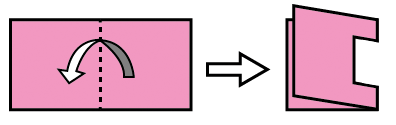
\includegraphics[scale=0.4]{cat-1}
		\vspace*{-10pt}
	\end{figure}
Em có biết khi mở tờ giấy ra, Bi nhận được hình nào trong những hình sau hay không?
\begin{figure}[H]
	\centering
	\captionsetup{labelformat=empty}
	\vspace*{-5pt}
	\captionsetup{justification=centering}
	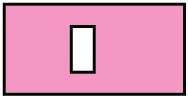
\includegraphics[width =0.16\textwidth]{cat-2a.jpeg}\quad
	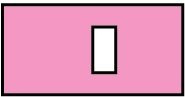
\includegraphics[width =0.16\textwidth]{cat-2b.jpeg}\quad
	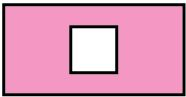
\includegraphics[width =0.16\textwidth]{cat-2c.jpeg}\quad
	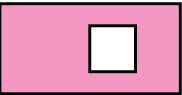
\includegraphics[width =0.16\textwidth]{cat-2d.jpeg}\quad
	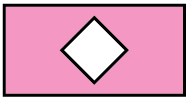
\includegraphics[width =0.16\textwidth]{cat-2e}
	\caption{\small\textit{(A) \hspace*{45pt} (B) \hspace*{45pt} (C) \hspace*{45pt} (D) \hspace*{45pt} (E)}}
	\vspace*{-5pt}
\end{figure}

Nếu còn nhớ về  tính đối xứng của hình vuông, các em sẽ thấy hình (\textit{C}) chính là đáp án đúng. Các em có thể dùng kéo và giấy để thử xem kết quả có đúng vậy không. Hãy cùng Bi thử với một hình phức tạp hơn nhé.
\vskip 0.1cm
\begin{multicols}{2}
	\textbf{Câu hỏi $\pmb{1}$:} Bi gập đôi một tờ giấy lại và cắt bỏ một phần để phần còn lại là hình bên:
	
	\columnbreak
	\begin{figure}[H]
		\centering
		\captionsetup{labelformat=empty}
		\vspace*{-5pt}
		\captionsetup{justification=centering}
		
\includegraphics[width =0.2\textwidth]{cat-3}
		\vspace*{-10pt}
	\end{figure}
\end{multicols}
Hỏi khi mở tờ giấy ra, Bi đã nhận được hình nào trong các hình dưới đây (đường nét đứt là đường gập đôi)?
\begin{figure}[H]
	\centering
	\captionsetup{labelformat=empty}
	\vspace*{-5pt}
	\captionsetup{justification=centering}
	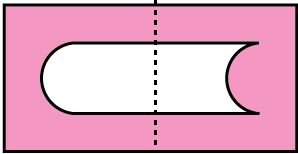
\includegraphics[width =0.2\textwidth]{cat-3a.jpeg}\quad
	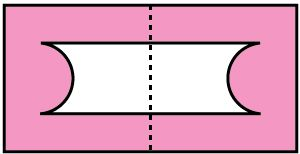
\includegraphics[width =0.2\textwidth]{cat-3b.jpeg}\quad
	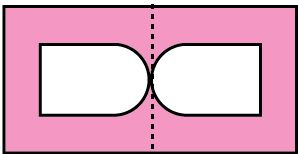
\includegraphics[width =0.2\textwidth]{cat-3c.jpeg}\quad
	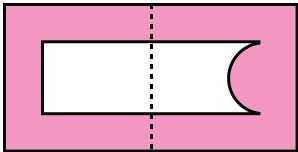
\includegraphics[width =0.2\textwidth]{cat-3d.jpeg}
	\caption{\small\textit{(A) \hspace*{55pt} (B) \hspace*{55pt}(C) \hspace*{55pt} (D)}}
	\vspace*{-10pt}
\end{figure}
Từ đó, Bi thấy, nếu muốn cắt được một hình đối xứng, Bi có thể gập đôi tờ giấy lại để cắt. Vậy là Bi đến đố các bạn trong lớp.
\vskip 0.1cm
\textbf{Câu hỏi $\pmb{2}$:} Bi gập đôi một tờ giấy lại và đố Ly cắt ra hình trái tim.
\begin{figure}[H]
	\centering
	\captionsetup{labelformat=empty}
	\vspace*{-5pt}
	\captionsetup{justification=centering}
	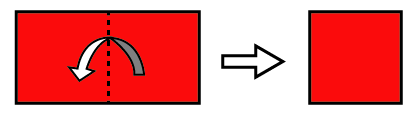
\includegraphics[width =0.65\textwidth]{cat-4}
	\vspace*{-10pt}
\end{figure}
Hỏi Ly cần phải cắt như thế nào để có hình trái tim ở trên?
\begin{figure}[H]
	\centering
	\captionsetup{labelformat=empty}
	\vspace*{-4pt}
	\captionsetup{justification=centering}
	
\includegraphics[width =0.1\textwidth]{cat-4a}
	\hfill
	
\includegraphics[width =0.1\textwidth]{cat-4b}
	\hfill
	
\includegraphics[width =0.1\textwidth]{cat-4c}
	\hfill
	
\includegraphics[width =0.1\textwidth]{cat-4d}
	\vspace*{-5pt}
	\caption{\small \it (A)\hspace*{75pt} (B)\hspace*{75pt} (C) \hspace*{75pt} (D)}
	\vspace*{-10pt}
\end{figure}
\begin{multicols}{2}
	Để cắt một hình vuông, ở trên, Bi đã gập đôi và cần ba nhát cắt (mỗi nhát ở đây được coi là một lần cắt thẳng). Tuy nhiên, với một lần gập đôi, và quan sát kĩ hình vuông, Bi chỉ cần hai nhát cắt để có được hình vuông: 
	
	\columnbreak
	\begin{figure}[H]
		\captionsetup{labelformat=empty}
		\vspace*{20pt}
		\centering
		\captionsetup{justification=raggedleft}
		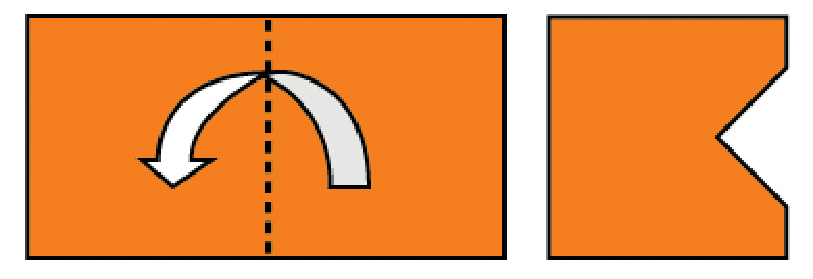
\includegraphics[width =0.44\textwidth]{cat-5}
		\vspace*{-5pt}
	\end{figure}
\end{multicols}
%\insertpic{195}{710}{.7}{../gapvacathinh/arrow}
%\insertpic{40}{700}{.35}{cat-4}
%\insertpic{228}{700}{.45}{cat-4them}
Em hãy thử suy nghĩ xem, với một lần gập đôi, liệu Bi có thể chỉ dùng một nhát cắt mà có  được hình vuông hay không? Với điều kiện khi cắt xong, ngoài hình vuông nhận được thì tờ giấy cũ vẫn còn liền nhau (không bị chia nhỏ).
\vskip 0.1cm
\begin{multicols}{2}
	\textbf{Câu hỏi $\pmb{3}$:} Từ một miếng giấy, để cắt được đúng một chú bướm như hình dưới đây, em có thể gập đôi nhiều nhất mấy lần để cắt?
	
	\columnbreak
	\begin{figure}[H]
		\captionsetup{labelformat=empty}
		\vspace*{-5pt}
		\centering
		\captionsetup{justification=raggedleft}
		
\includegraphics[width =0.3\textwidth]{cat-6}
	\end{figure}
\end{multicols}

Sau một vài lần thử gập một lần, Bi chuyển sang gập tờ giấy hai lần để khám phá và tìm ra các câu đố mới cho các bạn trong lớp.
\vskip 0.1cm
Bi đã gập đôi tờ giấy hai lần như hình bên dưới. Sau đó, Bi cắt một góc của tờ giấy: 
\begin{figure}[H]
	\captionsetup{labelformat=empty}
	\vspace*{5pt}
	\centering
	\captionsetup{justification=raggedleft}
	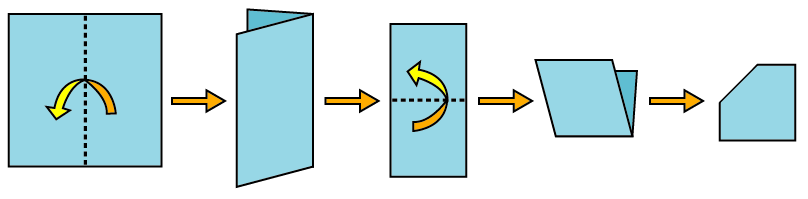
\includegraphics[width =0.85\textwidth]{cat-7a}
\end{figure}
\textbf{a)} Khi mở tờ giấy ra một lần, Bi thu được hình nào dưới đây?
\begin{figure}[H]
	\centering
	\captionsetup{labelformat=empty}
	\vspace*{-4pt}
	\captionsetup{justification=centering}
	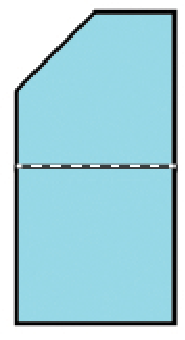
\includegraphics[width =0.08\textwidth]{cat-8a}
	\hfill
	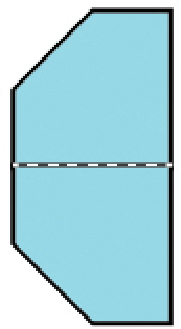
\includegraphics[width =0.08\textwidth]{cat-8b}
	\hfill
	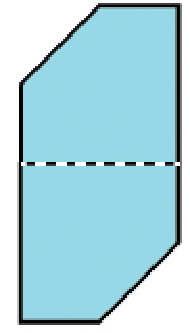
\includegraphics[width =0.08\textwidth]{cat-8c}
	\hfill
	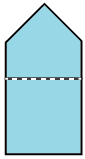
\includegraphics[width =0.08\textwidth]{cat-8d}
	\hfill
	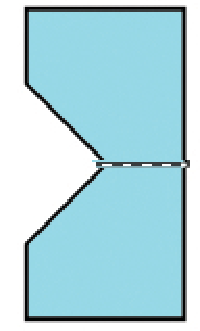
\includegraphics[width =0.08\textwidth]{cat-8e}	
	\caption{\small \it (A)\hfill (B) \hfill (C) \hfill (D) \hfill (E)}
	\vspace*{-10pt}
\end{figure}

\textbf{b)} Khi mở tờ giấy ra hai lần, Bi thu được hình nào dưới đây?
\begin{figure}[H]
	\centering
	\captionsetup{labelformat=empty}
	\vspace*{-5pt}
	\captionsetup{justification=centering}
	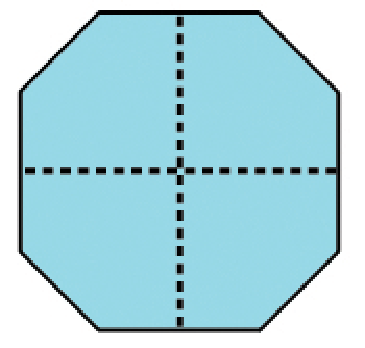
\includegraphics[width =0.19\textwidth]{cat-9a}
	\hfill
	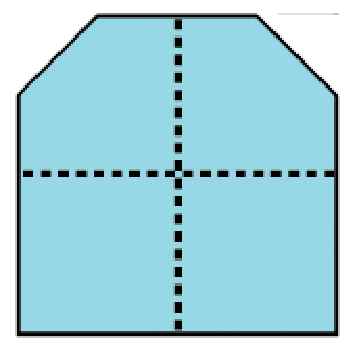
\includegraphics[width =0.19\textwidth]{cat-9b}
	\hfill
	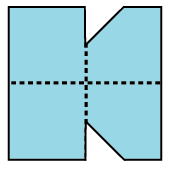
\includegraphics[width =0.19\textwidth]{cat-9c}
	\hfill
	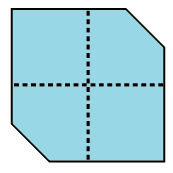
\includegraphics[width =0.19\textwidth]{cat-9d}
	\caption{\small \it (A) \hfill (B) \hfill (C) \hfill (D) \hfill (E)}
\end{figure}
Các em có tìm được câu trả lời không? Mình có thể làm từ từ từng bước đấy. Với câu a), đường đứt ở giữa là vết gập khi mở lần đầu tiên. Và dựa vào tính đối xứng, đáp án của câu a) chính là hình ($B$).
\vskip 0.1cm
Sau khi mở ra lần hai, đường đứt nằm dọc chính là vết gập khi mở lần hai. Đáp án của câu b) chính là hình (\textit{A}).
\vskip 0.1cm
Hình vuông có bốn trục đối xứng. Khi gập đôi một lần, Bi thấy để cắt rời hình vuông ra khỏi một tờ giấy, Bi cần cắt ba nhát hoặc hai nhát. Bây giờ, với hai lần gập giấy, liệu số nhát cắt cần thiết có ít đi hay không?
\vskip 0.1cm
\textbf{Câu hỏi $\pmb{4}$:} Bi gập đôi tờ giấy hai lần như hình bên dưới. 
\begin{figure}[H]
	\captionsetup{labelformat=empty}
	\vspace*{-5pt}
	\centering
	\captionsetup{justification=raggedleft}
	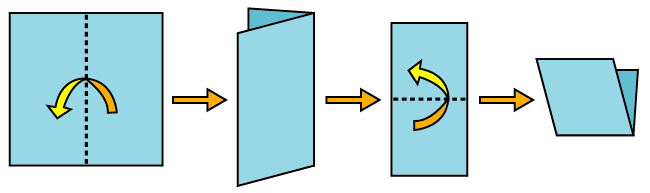
\includegraphics[width =0.7\textwidth]{cat-10}
	\vspace*{-10pt}
\end{figure}
Sau đó, Bi đã đố My chỉ bằng một nhát cắt, hãy cắt ra một hình vuông. Hỏi My nên cắt như thế nào?
\begin{figure}[H]
	\vspace*{-5pt}
	\centering
	\captionsetup{labelformat=empty}
	\captionsetup{justification=centering}
	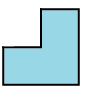
\includegraphics[width =0.2\textwidth]{cat-10a}
	\hfill
	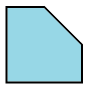
\includegraphics[width =0.2\textwidth]{cat-10b}
	\hfill
	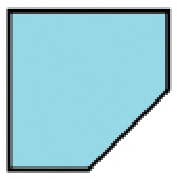
\includegraphics[width =0.2\textwidth]{cat-10c}
	\hfill
	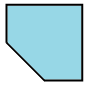
\includegraphics[width =0.2\textwidth]{cat-10d}	
	\vspace*{-5pt}
	\caption{\small \it (A)\hspace*{40pt} (B)\hspace*{65pt} (C) \hspace*{40pt} (D)}
	\vspace*{-10pt}
\end{figure}
\begin{multicols}{2}
	Bi biết là các bạn gái rất thích cắt hoa. Thế là Bi đố Ly cắt bông hoa bốn cánh.
	
	\columnbreak
	\begin{figure}[H]
		\vspace*{-5pt}
		\captionsetup{labelformat=empty}
		\centering
		\captionsetup{justification=raggedleft}
		
\includegraphics[width =0.2\textwidth]{cat-11}
		\vspace*{-10pt}
	\end{figure}
\end{multicols}
\textbf{Câu hỏi $\pmb{5}$:} Bi gập đôi tờ giấy hai lần như hình bên dưới.
\begin{figure}[H]
	\vspace*{-5pt}
	\captionsetup{labelformat=empty}
	\centering
	\captionsetup{justification=raggedleft}
	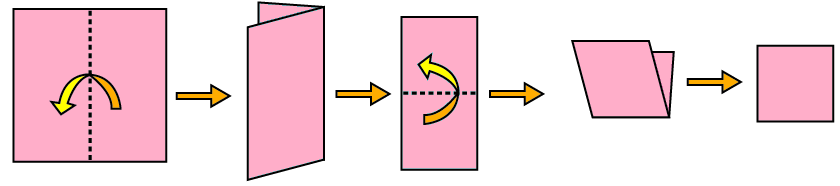
\includegraphics[width =1\textwidth]{cat-12}
	\vspace*{-10pt}
\end{figure}
Ly nên cắt tờ giấy (đã được gập) như thế nào để có được bông hoa bốn cánh ở trên?
\begin{figure}[H]
	\centering
	\captionsetup{labelformat=empty}
	\vspace*{-5pt}
	\captionsetup{justification=centering}
	
\includegraphics[width =0.2\textwidth]{cat-13a}
	\hfill
	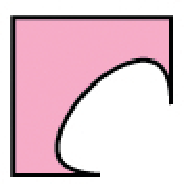
\includegraphics[width =0.2\textwidth]{cat-13b}
	\hfill
	
\includegraphics[width =0.2\textwidth]{cat-13c}
	\hfill
	
\includegraphics[width =0.2\textwidth]{cat-13d}	
	\vspace*{-5pt}
	\caption{\small \it (A)\hspace*{40pt} (B)\hspace*{65pt} (C) \hspace*{40pt} (D)}
	\vspace*{-10pt}
\end{figure}
Ly đã trả lời đúng câu đố của Bi đấy. Nhưng sau đó, Ly thấy rằng, nếu gập thêm một lần nữa thì sẽ cắt bông hoa còn nhanh hơn cơ.
\vskip0.25cm
\textbf{Câu hỏi $\pmb{6}$:} Từ mảnh giấy hình tròn, Ly gập đôi mảnh giấy ba lần như hình bên dưới: 
\begin{figure}[H]
	\vspace*{-10pt}
	\captionsetup{labelformat=empty}
	\centering
	\captionsetup{justification=raggedleft}
	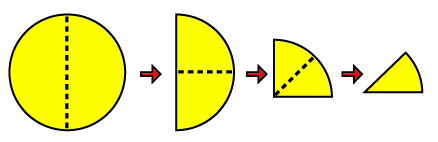
\includegraphics[width =0.85\textwidth]{cat-14}
\end{figure}	
Ly  đã cắt như thế nào để có được hình bông hoa bốn cánh?
\begin{figure}[H]
	\centering
	\captionsetup{labelformat=empty}
	\vspace*{-10pt}
	\captionsetup{justification=centering}
	
\includegraphics[width =0.2\textwidth]{cat-15a}
	\hfill
	
\includegraphics[width =0.2\textwidth]{cat-15b}
	\hfill
	
\includegraphics[width =0.2\textwidth]{cat-15c}
	\hfill
	
\includegraphics[width =0.2\textwidth]{cat-15d}	
	\caption{\small \it (A)\hspace*{40pt} (B)\hspace*{65pt} (C) \hspace*{40pt} (D)}
	\vspace*{-10pt}
\end{figure}
Từ đó, em hãy suy nghĩ xem, nếu cắt bông hoa sáu cánh, tám cánh, thì làm như thế nào sẽ cắt được bông hoa có các cánh đều nhất và nhanh nhất nhé. Và nếu muốn cắt hình lục giác đều, ngũ giác đều, thì nên làm như thế nào? 
\begin{figure}[H]
	\centering
	\captionsetup{labelformat=empty}
%	\vspace*{-5pt}
	\captionsetup{justification=centering}
	
\includegraphics[width =0.2\textwidth]{cat-16a}
	\hfill
	
\includegraphics[width =0.2\textwidth]{cat-16b}
	\hfill
	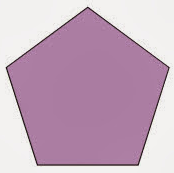
\includegraphics[width =0.2\textwidth]{cat-16c}
	\hfill
	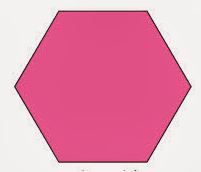
\includegraphics[width =0.2\textwidth]{cat-16d}	
	\vspace*{-5pt}
\end{figure}
Bây giờ, mình hãy cùng xem khi cắt hình phức tạp hơn một chút thì hình nhận được sẽ thế nào.
\vskip0.3cm
\textbf{Câu hỏi $\pmb{7}$:} Bi đã gập và cắt một mảnh giấy hình tròn như mô tả dưới đây:
\begin{figure}[H]
	\vspace*{-5pt}	
	\captionsetup{labelformat=empty}
	\centering
	\captionsetup{justification=raggedleft}
	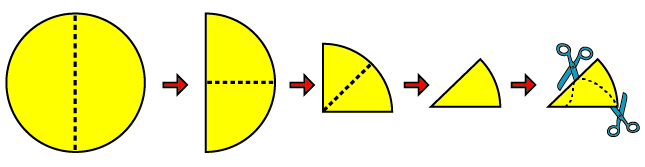
\includegraphics[width =1\textwidth]{cat-17}
	\vspace*{-10pt}
\end{figure}
Hỏi khi mở tờ giấy ra, bạn ấy sẽ thu được hình nào (bạn ấy giữ lại phần ở giữa)?
\begin{figure}[H]
	\centering
	\captionsetup{labelformat=empty}
	\vspace*{-5pt}
	\captionsetup{justification=centering}
	\includegraphics[width =0.2\textwidth]{cat-17a}
	\hfill
	\includegraphics[width =0.2\textwidth]{cat-17b}
	\hfill
	\includegraphics[width =0.2\textwidth]{cat-17c}
	\hfill
	\includegraphics[width =0.2\textwidth]{cat-17d}
	\caption{\small \it (A)\hspace*{40pt} (B)\hspace*{65pt} (C) \hspace*{40pt} (D)}	
	\vspace*{-10pt}
\end{figure}
\begin{multicols}{2}
	Hãy cùng làm những hình trang trí khác nhau từ cách cắt  hình mà chúng mình  đã khám phá cùng Bi ngày hôm nay nhé.
	\begin{figure}[H]
		\vspace*{-5pt}	
		\captionsetup{labelformat=empty}
		\centering
		\captionsetup{justification=raggedleft}
		\includegraphics[width =0.3\textwidth]{cat-18}
		\vspace*{-10pt}
	\end{figure}
\end{multicols}